\documentclass[11pt,a4paper]{article}

% ---------- Packages ----------
\usepackage[margin=2.3cm]{geometry}
\usepackage[T1]{fontenc}
\usepackage[utf8]{inputenc}
\usepackage{mathptmx}
\usepackage{microtype}
\usepackage{amsmath}
\usepackage{graphicx}
\usepackage{float}
\usepackage{booktabs}
\usepackage{array}
\usepackage{xcolor}
\usepackage{titlesec}
\usepackage{caption}
\usepackage{enumitem}
\usepackage{fancyhdr}
\usepackage[hidelinks]{hyperref}
\usepackage{tocloft}
\usepackage{needspace}
\emergencystretch=2em

% ---------- Style ----------
\definecolor{navy}{HTML}{1F3864}
\definecolor{steel}{HTML}{2F5496}
\setlength{\parindent}{0pt}
\setlength{\parskip}{6pt}
\renewcommand{\arraystretch}{1.25}

\titleformat{\section}{\Large\bfseries\color{navy}}{\thesection.}{0.6em}{}
\titleformat{\subsection}{\large\bfseries\color{steel}}{\thesubsection}{0.6em}{}
\titlespacing*{\section}{0pt}{16pt}{6pt}
\let\oldsection\section
\renewcommand{\section}{\Needspace{6\baselineskip}\oldsection}
\titlespacing*{\subsection}{0pt}{12pt}{4pt}

\captionsetup[figure]{font={small,it,color=gray},labelfont={small,it,color=gray},justification=centering,skip=4pt}
\captionsetup[table]{font=small,labelfont={bf,color=navy},textfont={bf,color=navy},justification=raggedright,singlelinecheck=false,skip=4pt}

\pagestyle{fancy}
\fancyhf{}
\renewcommand{\headrulewidth}{0pt}
\fancyfoot[C]{\thepage}

\setlength{\cftbeforesecskip}{3pt}
\setlength{\cftbeforesubsecskip}{0pt}
\renewcommand{\cftsecfont}{\bfseries}

\newcommand{\tn}[1]{\par\vspace{2pt}{\small\itshape #1}\par\vspace{4pt}}

\begin{document}

% ---------- Title block (cover page removed) ----------
\begin{center}
  {\Large\bfseries\color{navy} The Geopolitics of Oil:\\[2pt]
  Macroeconomic Impact of the 2026 Gulf Crisis on\\[2pt]
  Advanced Net-Importing Economies}\\[6pt]
  {\small\scshape Advanced Econometrics Project --- Tunis Business School}
\end{center}
\vspace{4pt}

\tableofcontents
\newpage

% =====================================================
\section{Introduction}
The 2026 Gulf Crisis, ignited on February 27, 2026, delivered one of the sharpest geopolitical shocks to global energy markets in recent history. The ensuing disruption to Brent crude oil supply triggered immediate inflationary pressures across oil-importing economies. This project investigates the macroeconomic transmission of this shock to consumer price inflation in four advanced net-importing economies --- France, Germany, Italy, and Japan --- using monthly panel data spanning February 2023 to May 2026.

These four countries constitute a theoretically coherent comparison group: all are large, institutionally developed economies, none produces significant domestic crude oil, all are deeply integrated into global trade and financial markets, and three of the four (France, Germany, Italy) share the same monetary authority (the European Central Bank). This homogeneity ensures that cross-country differences are attributable to structural and cyclical factors rather than incomparable institutional frameworks.

Using a balanced panel of 160 observations (4 countries $\times$ 40 months), we estimate Pooled OLS, Fixed Effects (FE), and Random Effects (RE) models with the natural log of CPI as the primary dependent variable, and $\ln(\text{IPI})$ as a secondary dependent variable to test for stagflationary output effects. Diagnostic tests select the Fixed Effects estimator. The main finding is that the post-crisis period is associated with a modest but statistically significant increase in CPI within individual countries (about $+0.96\%$, $p=0.038$) after controlling for macroeconomic fundamentals, while the policy rate and the nominal effective exchange rate are the most strongly significant within-country correlates of inflation. The oil price shock itself is not statistically significant, and the IPI model finds no statistically significant output effects.

% =====================================================
\section{Theoretical Framework}
For advanced net-importing economies, the transmission of oil price shocks to inflation operates through two principal channels. The direct channel works through the energy component of the CPI basket: higher imported fuel prices raise household heating and transportation costs immediately. The indirect channel operates through production costs: energy-intensive industries pass higher input costs onto consumers through pricing, amplifying the initial shock.

In the Eurozone context (France, Germany, Italy), an additional dimension arises: the ECB's single monetary policy implies that individual member countries cannot independently adjust their nominal interest rates in response to country-specific inflation differentials. For Japan, the prolonged near-zero interest rate environment (0.3\% throughout the sample period) creates a distinct monetary transmission dynamic.

\subsection{Panel Model Specification}
The core specification is a one-way Fixed Effects model with entity (country) effects:
\[
\ln(\text{CPI}_{it}) = \alpha_i + \beta_1\,\text{OilShock}_t + \beta_2\,\ln(\text{NEER}_{it}) + \beta_3\, r_{it} + \beta_4\,\text{VIX}_t + \beta_5\,\text{PostCrisis}_t + \varepsilon_{it}
\]
The country fixed effects $\alpha_i$ absorb all time-invariant unobserved heterogeneity. The within estimator identifies coefficients exclusively from time-series variation within each country, removing all cross-sectional confounds.

\subsection{Variable Definitions and Expected Signs}
\begin{table}[H]
\caption{Variable Definitions, Expected Signs, and Data Sources}
\centering\small
\begin{tabular}{|p{2.6cm}|p{2.1cm}|p{1.7cm}|p{4.8cm}|p{2.5cm}|}
\hline
\textbf{Variable} & \textbf{Symbol} & \textbf{Expected Sign} & \textbf{Description} & \textbf{Source}\\\hline
Inflation (Dep.) & $\ln(\text{CPI}_{it})$ & --- & Log CPI (2015=100) & IMF IFS / OECD\\\hline
Growth (Dep.) & $\ln(\text{IPI}_{it})$ & --- & Log Industrial Production Index (2015=100) & IMF IFS / FRED\\\hline
Oil Shock & $\text{OilShock}_t$ & $+$ (CPI), $-$ (IPI) & \% change in Brent crude price & U.S. EIA / FRED\\\hline
Exchange Rate & $\ln(\text{NEER}_{it})$ & $-$ & Log Nominal Effective Exchange Rate & BIS / FRED\\\hline
Policy Rate & $r_{it}$ & $-$ & Central bank policy rate (\%) & BIS / National CBs\\\hline
Global Risk & $\text{VIX}_t$ & $+$ (CPI), $-$ (IPI) & CBOE Volatility Index & FRED (VIXCLS)\\\hline
Post-Crisis & $\text{PostCrisis}_t$ & $+$ & $=1$ if date $\ge$ March 2026 & Authors' construction\\\hline
\end{tabular}
\end{table}

% =====================================================
\section{Data and Sample Construction}
\subsection{Country Selection and Justification}
The sample is restricted to the Advanced Net-Importers group as defined in the project guidelines. This homogeneous group ensures comparability of macroeconomic structures and policy responses.

\begin{table}[H]
\caption{Panel Composition --- Advanced Net-Importers}
\centering\small
\begin{tabular}{|p{2cm}|p{3.6cm}|p{8cm}|}
\hline
\textbf{Country} & \textbf{Role} & \textbf{Key Characteristics}\\\hline
France & Advanced Net-Importer & Highly energy-dependent; ECB monetary policy; CPI range 115.8--121.6\\\hline
Germany & Advanced Net-Importer & Largest EU economy; export-oriented; CPI range 121.5--127.8\\\hline
Italy & Advanced Net-Importer & High inflation vulnerability; fiscal constraints; CPI range 118.8--125.6\\\hline
Japan & Advanced Net-Importer & Near-zero policy rate (0.3\%); yen sensitivity; CPI range 106.3--115.7\\\hline
\end{tabular}
\end{table}

\subsection{Sample Period and Variables}
The sample spans February 2023 to May 2026, yielding 40 monthly observations per country (160 total). All CPI and IPI series use a 2015=100 base with the exception of Japan's CPI, which is sourced from the IMF IFS (series JPN.CPI.\_T.IX.M) on a 2020=100 base. This level difference is fully absorbed by Japan's country fixed effect in the FE estimator and does not affect slope coefficient estimates. Japan's CPI is observed through March 2026 and extended to May 2026 using ARIMA(1,1,1)(1,1,1)$_{12}$ seasonal forecasts; Japan's IPI values for March--May 2026 are filled in the same way. Japan's CPI shows meaningful variation over the sample (106.3 in Feb 2023 rising to 115.7 by May 2026).

\subsection{Descriptive Statistics}
\begin{table}[H]
\caption{Descriptive Statistics --- Full Panel (N=160)}
\centering\small
\begin{tabular}{|l|r|r|r|r|r|}
\hline
\textbf{Variable} & \textbf{Mean} & \textbf{Std. Dev.} & \textbf{Min} & \textbf{Median} & \textbf{Max}\\\hline
CPI (2015=100) & 119.67 & 5.65 & 106.30 & 120.40 & 127.78\\\hline
IPI (2015=100) & 96.18 & 4.09 & 88.76 & 97.19 & 104.55\\\hline
NEER (2015=100) & 92.29 & 11.81 & 65.70 & 98.49 & 101.20\\\hline
OilShock (\%) & 1.10 & 9.29 & $-$10.84 & $-$0.61 & 45.49\\\hline
VIX & 16.76 & 3.18 & 12.44 & 16.58 & 25.25\\\hline
Policy Rate (\%) & 2.32 & 1.36 & 0.30 & 2.25 & 4.00\\\hline
\end{tabular}
\end{table}

\begin{table}[H]
\caption{Descriptive Statistics by Country}
\centering\small
\begin{tabular}{|l|r|r|r|r|r|}
\hline
\textbf{Country} & \textbf{CPI Mean} & \textbf{CPI Std} & \textbf{IPI Mean} & \textbf{IPI Std} & \textbf{Rate Mean}\\\hline
France & 119.63 & 1.40 & 98.45 & 0.55 & 2.99\\\hline
Germany & 125.91 & 1.95 & 92.03 & 1.51 & 2.99\\\hline
Italy & 121.64 & 1.89 & 101.40 & 1.05 & 2.99\\\hline
Japan & 111.51 & 2.93 & 92.82 & 1.47 & 0.30\\\hline
\end{tabular}
\end{table}

Japan's CPI mean of 111.51 is meaningfully lower than the European peers (France 119.63, Germany 125.91, Italy 121.64), reflecting Japan's distinct price-level and monetary policy environment. The CPI standard deviation of 2.93 for Japan confirms genuine time variation in the series --- essential for valid Fixed Effects identification.

% =====================================================
\section{Exploratory Data Analysis}
\begin{figure}[H]
\centering
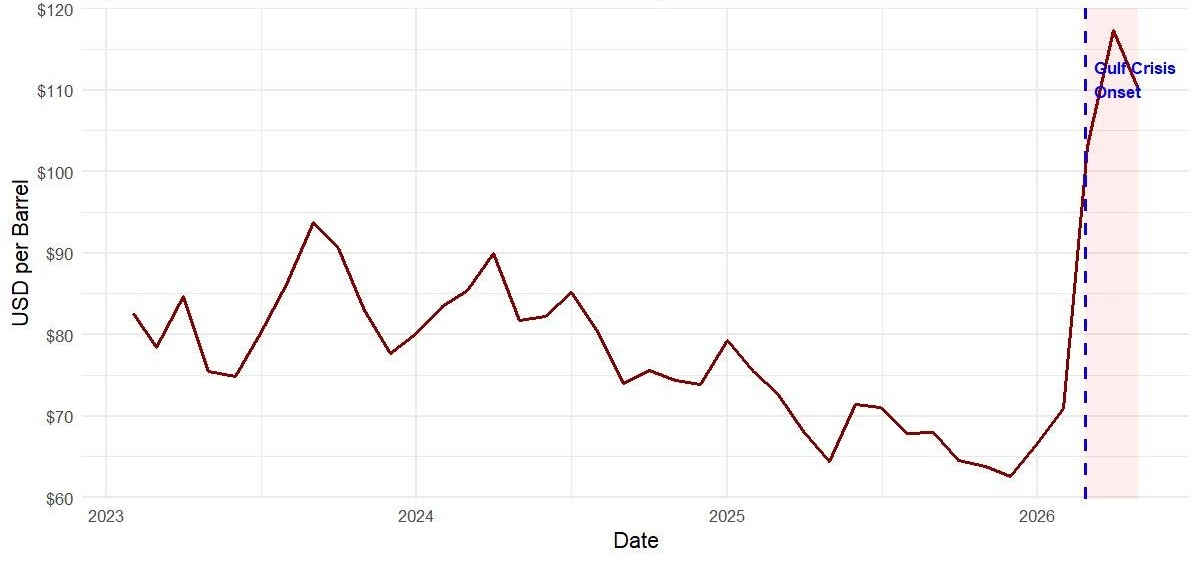
\includegraphics[width=\linewidth]{figures/fig1_brent.jpg}
\caption{Monthly Brent crude oil price (USD/barrel). The dashed line marks the Gulf Crisis onset (Feb 27, 2026). The March 2026 spike ($+45.5\%$) is the primary external shock of interest.}
\end{figure}

\begin{figure}[H]
\centering
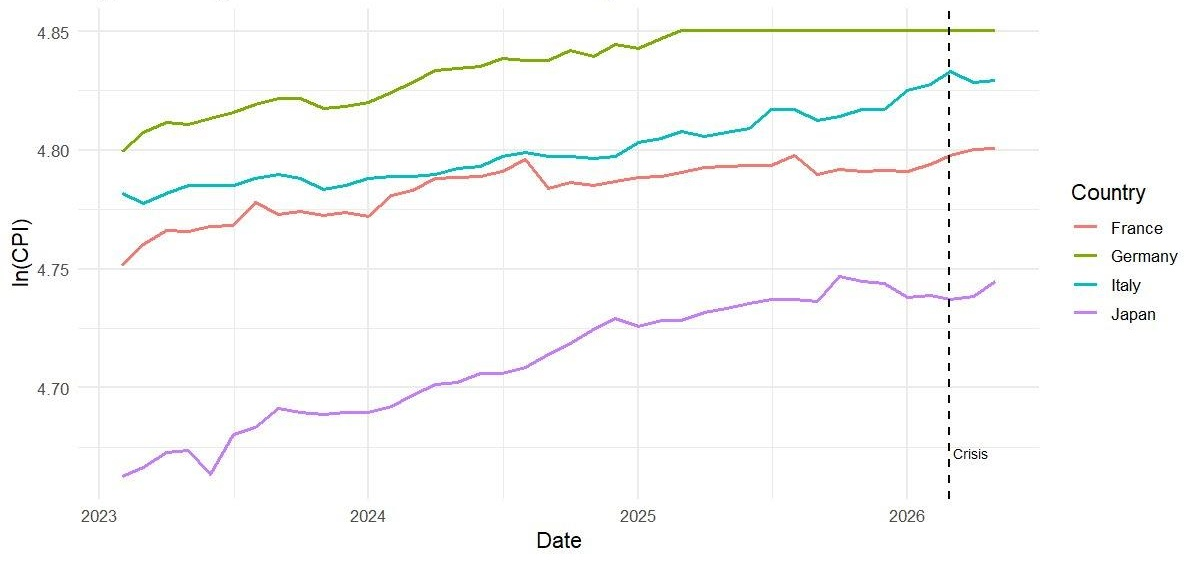
\includegraphics[width=\linewidth]{figures/fig2_cpi.jpg}
\caption{Individual $\ln(\text{CPI})$ series for France, Germany, Italy, and Japan. Japan's lower-level upward trajectory reflects its gradual inflation recovery and near-zero policy rate. France, Italy, and Japan edge upward around the crisis onset in March 2026, while Germany's series is flat.}
\end{figure}

\begin{figure}[H]
\centering
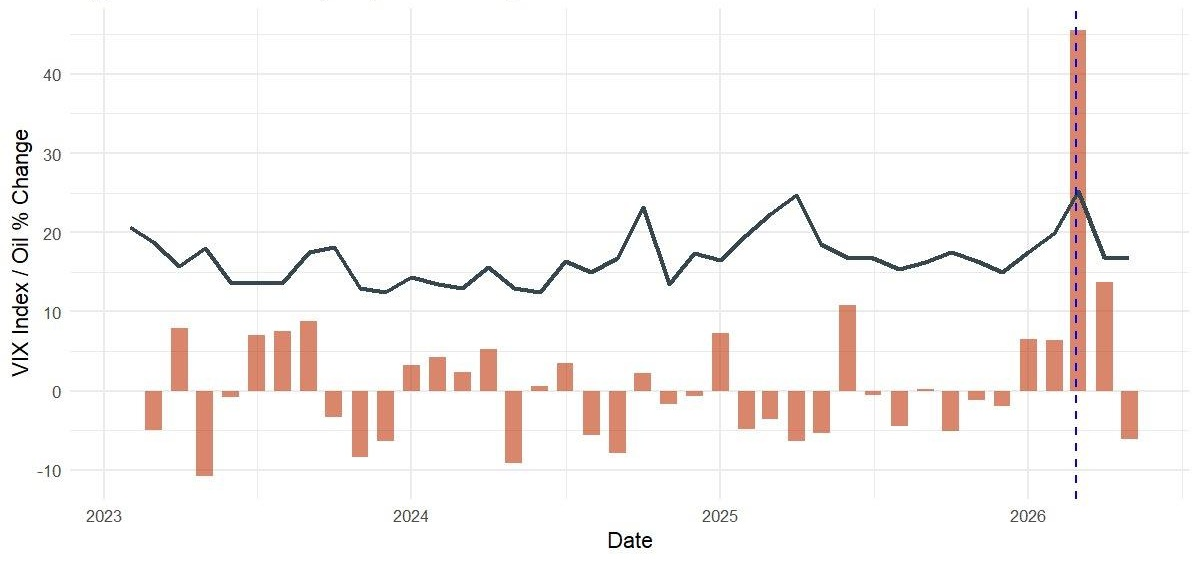
\includegraphics[width=\linewidth]{figures/fig3_vix_oil.jpg}
\caption{VIX index (line) and monthly Brent crude \% change (bars). Co-movement of global risk and oil price volatility around February 2026 justifies their joint inclusion in the regression.}
\end{figure}

\begin{figure}[H]
\centering
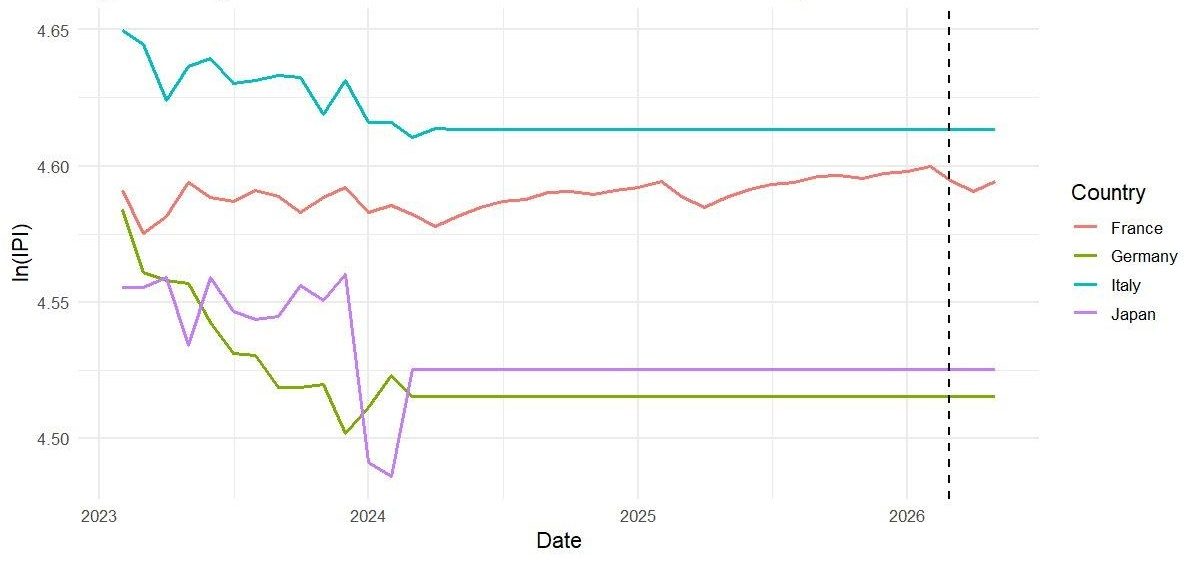
\includegraphics[width=\linewidth]{figures/fig4_ipi.jpg}
\caption{Individual $\ln(\text{IPI})$ series. Germany's industrial production declines through early 2024. Only France shows a small dip after the crisis onset; the series for Germany, Italy, and Japan are flat from early 2024 onward, so the figure offers little visual evidence of a post-crisis output effect.}
\end{figure}

% =====================================================
\section{Econometric Methodology}
\subsection{The Three Estimators}
\textbf{Pooled OLS.} Pooled OLS treats all 160 observations as a homogeneous cross-section. Given Japan's structurally different CPI level (mean 111.51 vs.\ European average $\sim$122.4) and monetary regime (0.3\% vs.\ ECB's 2--4\%), the assumption that unobserved effects are uncorrelated with regressors is implausible.

\textbf{Fixed Effects (Within Estimator).} The Fixed Effects estimator introduces a separate intercept $\alpha_i$ for each country, absorbing Japan's structural CPI level difference. FE identifies coefficients exclusively from within-country time-series variation.

\textbf{Random Effects (GLS Estimator).} The Random Effects estimator treats country effects as random draws uncorrelated with the regressors. With only 4 panel units this estimator has limited degrees of freedom. The Hausman test provides the formal selection criterion.

\subsection{Diagnostic Tests}
\textbf{Breusch-Pagan LM Test:} Tests $H_0$: no individual effects (POLS is adequate).

\textbf{Hausman Test:} Tests $H_0$: country effects uncorrelated with regressors (RE efficient). Rejection mandates FE.

\textbf{Serial Correlation:} Per-entity DW statistics test for autocorrelation; rejection calls for Arellano HAC robust standard errors.

\textbf{Heteroskedasticity:} Tests $H_0$: homoskedastic residuals. Rejection also calls for HAC robust standard errors.

% =====================================================
\clearpage
\section{Empirical Results}
\subsection{Diagnostic Test Results}
\begin{table}[H]
\caption{Diagnostic Test Results}
\centering\small
\begin{tabular}{|p{4.6cm}|p{2.2cm}|p{2.4cm}|p{4.2cm}|}
\hline
\textbf{Test} & \textbf{Statistic} & \textbf{p-value} & \textbf{Conclusion}\\\hline
Breusch-Pagan (POLS vs RE) & $\chi^2=423.00$ & $<2.2\text{e-}16$ *** & RE preferred over Pooled OLS\\\hline
Hausman (FE vs RE) & $\chi^2=198.30$ & $<2.2\text{e-}16$ *** & FE preferred over RE\\\hline
Serial Correlation (Lag-1) & $F=8.84$ & 0.003 ** & HAC robust SE required\\\hline
Heteroskedasticity (BP) & $\chi^2=29.39$ & $<0.001$ *** & HAC robust SE required\\\hline
\end{tabular}
\end{table}

Breusch-Pagan ($\chi^2=423.00$) decisively rejects POLS. Hausman ($\chi^2=198.30$) strongly rejects RE, so Fixed Effects is the preferred estimator. Serial correlation ($F=8.84$) and heteroskedasticity ($\chi^2=29.39$) call for Arellano HAC robust standard errors throughout.

\subsection{CPI Model --- Three-Model Comparison}
\begin{table}[H]
\caption{Pooled OLS, Fixed Effects, and Random Effects --- CPI Model}
\centering\small
\begin{tabular}{|p{2.9cm}|p{1.9cm}|p{2.3cm}|p{1.9cm}|p{4.3cm}|}
\hline
\textbf{Variable} & \textbf{POLS} & \textbf{FE (Preferred)} & \textbf{RE} & \textbf{Note}\\\hline
\texttt{oil\_pct\_change} & $-$0.00004 & $-$0.00008 & $-$0.00004 & n/s across all models\\\hline
$\ln(\text{NEER})$ & 0.3660 *** & $-$0.3101 ** & 0.3660 *** & Sign reversal: FE removes cross-sectional bias\\\hline
\texttt{policy\_rate} & $-$0.0024 & $-$0.0092 ** & $-$0.0024 & FE identifies the within-country negative association\\\hline
\texttt{vix} & 0.0010 & 0.0005 & 0.0010 & n/s across all models\\\hline
\texttt{post\_crisis} & 0.0299 *** & 0.0096 * & 0.0299 *** & FE controls country-level heterogeneity\\\hline
$R^2$ & 0.7754 & 0.4070 (within) & 0.7754 & Balanced panel: N=160\\\hline
\end{tabular}
\end{table}

\subsection{Preferred Fixed Effects Model --- CPI Detailed Results}
\begin{table}[H]
\caption{Fixed Effects Regression --- CPI Model (Dependent Variable: ln CPI)}
\centering\small
\begin{tabular}{|l|r|r|r|r|c|}
\hline
\textbf{Variable} & \textbf{Coefficient} & \textbf{Robust Std. Err.} & \textbf{t-stat} & \textbf{p-value} & \textbf{Sig.}\\\hline
\texttt{oil\_pct\_change} & $-$0.000081 & 0.000126 & $-$0.646 & 0.519 & ---\\\hline
$\ln(\text{NEER})$ & $-$0.3101 & 0.0985 & $-$3.150 & 0.002 & **\\\hline
\texttt{policy\_rate} & $-$0.0092 & 0.0028 & $-$3.322 & 0.001 & **\\\hline
\texttt{vix} & 0.0005 & 0.0007 & 0.710 & 0.479 & ---\\\hline
\texttt{post\_crisis} & 0.0096 & 0.0046 & 2.095 & 0.038 & *\\\hline
\end{tabular}
\tn{Entity fixed effects included. Arellano HAC robust SE. $R^2$ (within) = 0.407. N=160. ** $p<0.01$, * $p<0.05$.}
\end{table}

Within countries, the policy rate and the exchange rate are the most strongly significant correlates of CPI. A one-percentage-point higher policy rate is associated with a CPI level about 0.92\% lower, a 1\% stronger nominal effective exchange rate is associated with a CPI level about 0.31\% lower, and the post-March-2026 period is associated with a CPI level about 0.96\% higher. The oil price change itself and the VIX are not statistically significant, so the crisis effect is captured by the post-crisis dummy rather than by the monthly oil price change.

\begin{figure}[H]
\centering
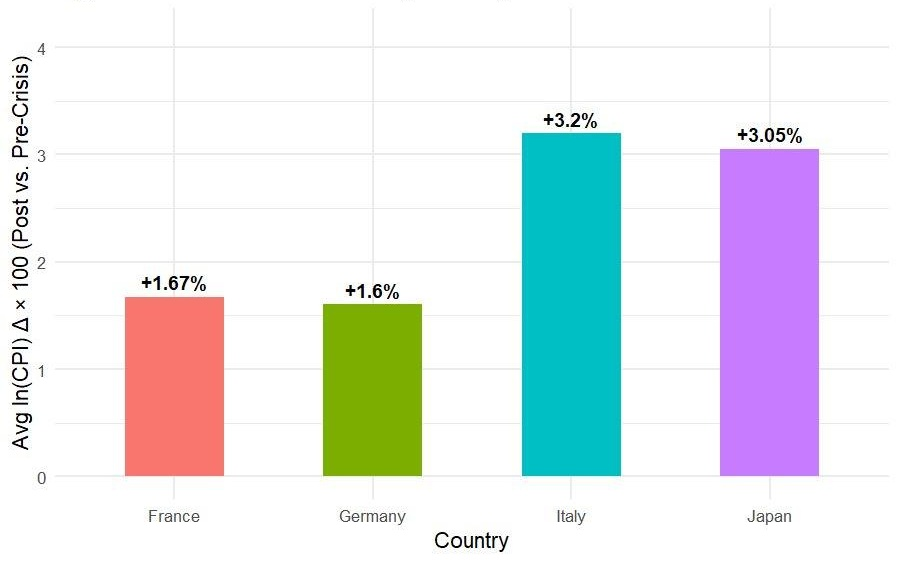
\includegraphics[width=0.92\linewidth]{figures/fig5_cpi_lift.jpg}
\caption{Post-crisis CPI lift by country. Japan ($+3.05\%$) and Italy ($+3.2\%$) register the largest lifts, consistent with limited monetary policy space and structural energy dependence respectively. Lifts are raw differences in average $\ln(\text{CPI})$ between the post- and pre-crisis windows, so they also reflect each series' pre-existing upward trend.}
\end{figure}

\begin{figure}[H]
\centering
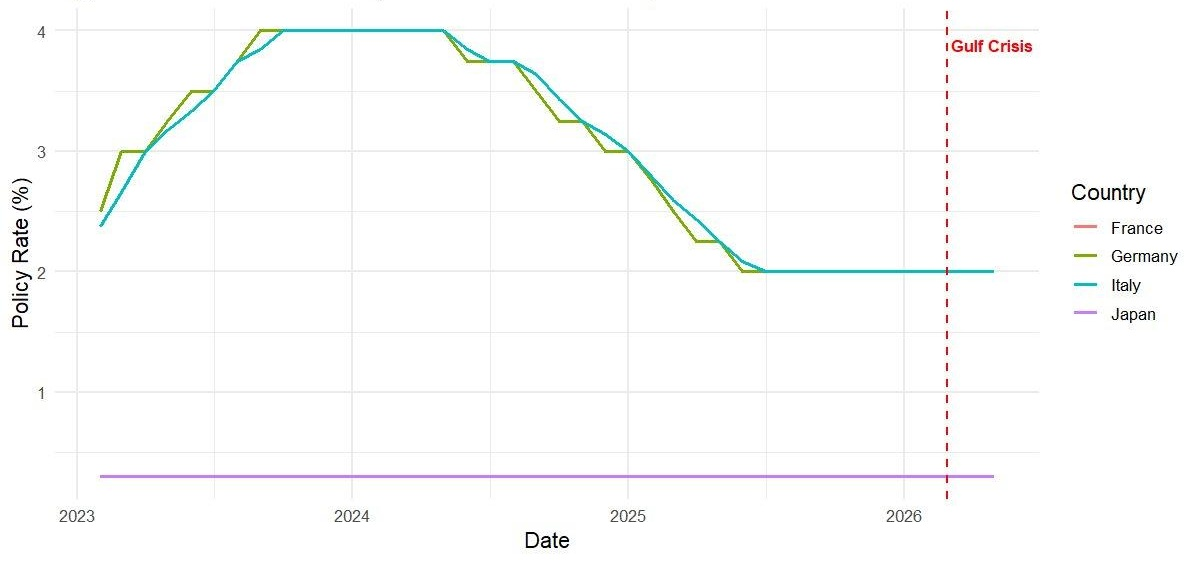
\includegraphics[width=0.92\linewidth]{figures/fig6_policy_rates.jpg}
\caption{Central bank policy rates. Japan's near-zero rate (0.30\%) is structurally distinct from the ECB's tightening-and-cutting cycle (peak 4.0\% in 2023--2024).}
\end{figure}

\subsection{IPI Model --- Testing for Stagflationary Output Effects}
\begin{table}[H]
\caption{Fixed Effects Regression --- IPI Model (Dependent Variable: ln IPI)}
\centering\small
\begin{tabular}{|l|r|r|r|r|c|}
\hline
\textbf{Variable} & \textbf{Coefficient} & \textbf{Robust Std. Err.} & \textbf{t-stat} & \textbf{p-value} & \textbf{Sig.}\\\hline
\texttt{oil\_pct\_change} & $-$0.000037 & 0.000126 & $-$0.296 & 0.768 & ---\\\hline
$\ln(\text{NEER})$ & 0.1274 & 0.0506 & 2.519 & 0.013 & *\\\hline
\texttt{policy\_rate} & $-$0.0003 & 0.0014 & $-$0.189 & 0.850 & ---\\\hline
\texttt{vix} & 0.0003 & 0.0006 & 0.403 & 0.687 & ---\\\hline
\texttt{post\_crisis} & $-$0.0009 & 0.0026 & $-$0.322 & 0.748 & ---\\\hline
\end{tabular}
\tn{Entity fixed effects included. Arellano HAC robust SE. $R^2$ (within) = 0.063. N=160. * $p<0.05$.}
\end{table}

The oil shock coefficient ($-0.000037$) and the post-crisis coefficient ($-0.0009$) have the negative sign expected for output, but neither is statistically distinguishable from zero. The VIX ($0.0003$, $p=0.687$) and policy rate ($-0.0003$, $p=0.850$) coefficients are also insignificant, and the within $R^2$ is only 0.063. The only significant coefficient is $\ln(\text{NEER})$ ($0.1274$, $p=0.013$). The opposite signs of the post-crisis effect in the CPI model ($+$) and the IPI model ($-$) are consistent in direction with a stagflationary narrative, but the IPI model provides no statistically significant evidence of an output effect over this short window.

% =====================================================
\section{Discussion and Policy Implications}
\subsection{Why Fixed Effects and Why Japan Matters}
Japan's CPI mean of 111.51 versus the European average of $\sim$122.4 represents a structural level difference. In POLS this contaminates all slope estimates. In FE Japan's individual intercept captures this difference, and slope estimates reflect only within-country dynamics. This is why the policy rate coefficient becomes statistically significant in FE ($-0.0092$, $p=0.001$) while it is insignificant in POLS ($-0.0024$), and why the $\ln(\text{NEER})$ coefficient changes sign from $+0.3660$ in POLS to $-0.3101$ in FE.

\subsection{Post-Crisis CPI Impact by Country}
Figure 5 reveals heterogeneity within the Advanced Importers group. Japan ($+3.05\%$) and Italy ($+3.20\%$) show the largest post-crisis CPI lifts, while France ($+1.67\%$) and Germany ($+1.60\%$) show more modest increases. Japan's larger lift is consistent with its limited monetary policy space (0.30\% rate). Italy's large lift reflects its structural energy import dependence and fiscal constraints. These figures are raw post-versus-pre differences and are not adjusted for the pre-existing upward trend in each series.

\subsection{Heterogeneity Note}
The project guidelines request a heterogeneity analysis comparing oil importers vs.\ exporters. Since our panel consists exclusively of Advanced Net-Importers this split analysis is not applicable within our group, as directed by the professor.

\subsection{Policy Implications}
The policy rate coefficient ($\beta=-0.0092$, $p=0.001$) indicates that, within countries, a one-percentage-point higher policy rate is associated with a CPI level about 0.92\% lower, which is consistent with the disinflationary role of the ECB's tightening cycle. This is an association rather than a causal estimate, since policy rates fell over most of the sample while CPI trended upward. Japan's near-zero rate environment leaves limited conventional policy space; exchange rate policy and forward guidance may be more relevant tools.

% =====================================================
\section{Limitations and Extensions}
\textbf{Small N (4 countries).} With only four panel units, the power of the Hausman test is limited, and Arellano robust standard errors rely on a large number of clusters. They may therefore be too small here, so p-values close to 5\% (for example the post-crisis dummy, $p=0.038$) should be read with caution.

\textbf{Short post-crisis window.} Only three post-crisis months (March--May 2026) are available, and Japan's final months are ARIMA forecasts rather than observed values (see Section 3.2). Japan's CPI is sourced from the IMF International Financial Statistics database (series JPN.CPI.\_T.IX.M, IMF IFS CPI 5.0.0).

\textbf{Trending series and raw lifts.} CPI enters in logs of levels with an upward trend, and the model has no time trend or time effects, so the post-crisis dummy and the policy rate may partly capture trends rather than crisis effects. The country lifts in Figure 5 are likewise raw differences.

\textbf{Data variation.} In the dataset, Germany's CPI appears constant from early 2025 and the IPI series for Germany, Italy, and Japan appear constant from early 2024 (Figures 2 and 4). This limits the within-country variation available to the estimators, and the IPI results in particular should be read as exploratory.

\textbf{Potential extensions.} Arellano-Bond GMM, local projections, interaction terms, country-specific trends or first differences.

% =====================================================
\section{Conclusion}
This project applied panel data econometrics to assess the macroeconomic impact of the 2026 Gulf Crisis on CPI and IPI in four advanced net-importing economies using 160 monthly observations (February 2023--May 2026). The diagnostic sequence (BP: $\chi^2=423.00$; Hausman: $\chi^2=198.30$; DW: $F=8.84$; Heteroskedasticity: $\chi^2=29.39$) selected Fixed Effects with Arellano HAC robust standard errors throughout.

The FE CPI model finds: (i) a post-crisis effect of $+0.96\%$ ($p=0.038$), significant at the 5\% level but based on only three post-crisis months; (ii) a one-percentage-point higher policy rate associated with a 0.92\% lower CPI ($p=0.001$); and (iii) a negative and significant $\ln(\text{NEER})$ coefficient, while the oil price change and the VIX are not significant. The FE IPI model finds no statistically significant effect of the oil shock, VIX, policy rate, or crisis dummy on industrial production (within $R^2=0.063$), so the stagflationary hypothesis receives directional but not statistical support. Japan's raw post-crisis CPI lift ($+3.05\%$) is among the largest in the panel, an illustration of the exposure of structurally low-rate economies to external inflationary shocks, although raw lifts also reflect pre-existing trends.

% =====================================================
\section{R Script Reference}
The well-commented R script used to produce all results in this report is submitted alongside this document as \texttt{Panel\_Project\_Complete.R}. All results are fully reproducible by running the script with the accompanying \texttt{panel\_data\_final.csv} dataset.

% =====================================================
\section*{References}
\addcontentsline{toc}{section}{References}
\subsection*{Data Sources}
\begin{itemize}[leftmargin=1.2em,itemsep=2pt]
  \item International Monetary Fund (IMF). International Financial Statistics (IFS). Accessed 2026.
  \item International Monetary Fund (IMF). International Financial Statistics (IFS), CPI series 5.0.0 --- JPN.CPI.\_T.IX.M (Japan, Consumer Price Index, Total, Index). Accessed May 2026.
  \item OECD. Monthly CPI and Industrial Production Indices (2015=100). Accessed 2026.
  \item U.S. Energy Information Administration (EIA). Brent Crude Oil Prices. FRED: DCOILBRENTEU. Accessed 2026.
  \item Federal Reserve Bank of St.\ Louis (FRED). CBOE Volatility Index. FRED: VIXCLS. Accessed 2026.
  \item Bank for International Settlements (BIS). Nominal Effective Exchange Rates. Accessed 2026.
  \item European Central Bank. ECB Deposit Facility Rate. FRED: ECBDFR. Accessed 2026.
  \item Bank of Japan. Policy Rate. FRED: IRSTCB01JPM156N. Accessed 2026.
\end{itemize}
\subsection*{Methodology}
\begin{itemize}[leftmargin=1.2em,itemsep=2pt]
  \item Arellano, M. (1987). Computing Robust Standard Errors for Within-Groups Estimators. \textit{Oxford Bulletin of Economics and Statistics}, 49(4), 431--434.
  \item Breusch, T.S., \& Pagan, A.R. (1980). The Lagrange Multiplier Test. \textit{Review of Economic Studies}, 47(1), 239--253.
  \item Hausman, J.A. (1978). Specification Tests in Econometrics. \textit{Econometrica}, 46(6), 1251--1271.
  \item Wooldridge, J.M. (2002). \textit{Econometric Analysis of Cross Section and Panel Data}. MIT Press.
  \item Croissant, Y., \& Millo, G. (2008). Panel Data Econometrics in R: The plm Package. \textit{Journal of Statistical Software}, 27(2).
\end{itemize}

\end{document}
